\documentclass[12pt]{article}
\usepackage{mathtools}
\usepackage{amssymb}
\usepackage{amsthm}
\usepackage{pgfplots}
\usepackage{tikz}
\usetikzlibrary{calc}
\usepackage{polski}
\usepackage[utf8]{inputenc}
\usepackage{geometry}
\usepackage{amsmath}
\usepackage{gensymb}
\usepackage{mnsymbol}
\usepackage{graphicx}
\usepackage{textgreek}
\usepackage{float}
\usepackage{caption}
\begin{document}
\newgeometry{tmargin=2cm,bmargin=2cm,lmargin=2cm,rmargin=2cm}
\section{Cel ćwiczenia}
Celem ćwiczenia było wyznaczenie modułu Younga dla różnych materiałów na podstawie pomiaru prędkości rozchodzenia się fali dźwiękowej w pręcie.
\section{Wstęp teorytyczny}
W ośrodkach sprężystych wytrącenie pewnego obszaru z położenia równowagi powoduje drgania wokół tego położenia. Gdy ciałem drgającym jest pewna część jednorodnego ośrodka, wtedy tracona energia nie jest rozpraszana bezładnie, lecz wprawiana w ruch drgający sąsiadujące części ośrodka, dzięki czemu drgania przenoszą się w przestrzeni i w czasie. Takie przenoszenie drgań nazywamy falą. W najprostszym przypadku jest to drganie harmoniczne, w którym wychylenie \newline z położenia równowagi zmienia się  w czasie następująco:
\begin{center}
\Large $A(t)=A_0cos(\omega{t})$,
\end{center}
gdzie $A_0$ to amplituda drgań (największe wychylenie), $\omega=\frac{2\pi}{T}$ to częstotliwość kątowa a $T$ to okres drgań. \newline
Wskutek sprężystości ośrodka zaburzenie to przenosi się do coraz dalszych obszarów z prędkością $v$ zależną od właściwości danego ośrodka. Zjawisko to nazywamy falą mechaniczną.
W punkcie oddalonym od źródła zaburzenia o $x$ drgania pojawiają się z opóźnieniem $t$. Ogólnie dla wszystkich punktów $x$ drgającego ośrodka możemy zapisać:
\begin{center}
\Large $A(t,x)=A_0cos(\omega(t\pm{\frac{x}{v}}))$
\end{center}
Równanie opisuje falę rozchodzącą się w kierunku dodatniej osi $x$ – znak minus we wzorze, \newline w przypadku rozchodzenia się fali w kierunku przeciwnym we wzorze – znak plus.
Długością fali nazywamy najmniejszą odległość między punktami drgającymi w jednakowych fazach. Jest ona równa drodze jaką określona faza przebędzie z prędkością $v$ w czasie $T$:
\begin{center}
\Large $\lambda=vT\;\;\;=>\;\;\;v=\lambda{f}$,
\end{center}
gdzie $\lambda$ to długość fali, $f=\frac{1}{T}$ to częstotliwość rozchodzenia drgań fali a $v$ to prędkość dźwięku \newline w danym ośrodku. Jest to wzór słuszny dla każdego typu fali. \newline
Powierzchnię utworzoną przez punkty, do których doszło w danej chwili zaburzenie nazywamy czołem fali. Fale mogą więc być płaskie (w przypadku gdy fala rozchodzi się w jednym kierunku) lub kuliste (gdy źródło wysyła energię drgania tak samo we wszystkich kierunkach). W zależności od kierunku drgań cząsteczek ośrodka względem kierunku rozchodzenia się fali, fale mogą być podłużne – cząstki drgają równolegle lub poprzeczne – cząstki drgają prostopadle do kierunku rozchodzenia się fali. Fale poprzeczne powstają w ośrodkach charakteryzujących się sprężystością postaci (sztywnością). Dla występowania fal podłużnych wystarczający jest warunek sprężystości objętości. W cieczach i gazach mogą rozchodzić się tylko fale podłużne. W ciałach stałych mogą występować również fale poprzeczne. \newline
Przez ten sam obszar przestrzeni mogą przebiegać niezależnie od siebie dwie (lub więcej) fale. Przemieszczenie cząstki ośrodka jest wtedy sumą przemieszczeń, jakie wywoływałyby poszczególne fale. Proces takiego dodawania przemieszczeń nazywamy superpozycją fal. Fizyczne zjawiska nakładania się dwóch lub więcej ciągów falowych określane są mianem interferencji fal. Fala wypadkowa ma tę samą częstość co fale składowe, lecz inną amplitudę. Jeżeli fale mają wszędzie takie same fazy, to amplituda fali wypadkowej jest dwa razy większa niż amplitudy fal składowych. Gdy spotykają się „szczyty” i „doliny” fal, następuje interferencja konstruktywna, czyli wzmocnienie fal. W przypadku gdy fazy fal różnią się o $\frac{n}{2}$ (lub nieparzystej wielokrotności $\frac{n}{2}$), to „szczyt” jednej fali spotyka się z „doliną” drugiej, następuje wygaszenie i mamy do czynienia z interferencją destruktywną. Jeśli fale rozchodzą się w ośrodku o skończonych rozmiarach, to odbijają się one od granic takiego ośrodka, a po odbiciu poruszają się w kierunku przeciwnym niż fale padające, lecz posiadają w dalszym ciągu te same amplitudy i częstości co fale padające. Zgodnie z zasadą superpozycji fala padająca i odbita dodają się do siebie a powstała fala nosi nazwę fali stojącej,\newline  w której amplituda drgań cząstek ośrodka zależy od ich położenia w przestrzeni (nie jest taka sama dla wszystkich cząstek drgającego ośrodka) i dana jest wzorem: 
\begin{center}
\Large $A(x)=2A_0cos(2\pi\frac{x}{\lambda})$
\end{center}
Amplituda przyjmuje wartość maksymalną w punktach, dla których $x=n\frac{\lambda}{2}$, (gdzie: $n = 0, \pm1, \pm2$..) nazywamy je strzałkami fali, a odległość między nimi jest równa połowie długości fali, czyli $\frac{\lambda}{2}$ . Wartość amplitudy spada do zera w punktach, dla których 
$=(n+\frac{1}{2})\frac{\lambda}{2}$ , (gdzie: $n = 0, \pm1, \pm2$..) nazywamy je węzłami fali. Odległość pomiędzy dwoma sąsiednimi węzłami fali wynosi również połowę długości fali $\frac{\lambda}{2}$, natomiast pomiędzy sąsiednim węzłem i strzałką fali ćwierć długości fali $\frac{\lambda}{4}$. \newline
Podstawowym warunkiem powstania dobrze określonego obrazu interferencyjnego jest, aby interferujące fale świetlne miały dokładnie określoną różnicę faz
$\varphi$ stałą w czasie. Przypomnijmy, że faza określa stan fali w danym miejscu i czasie. 
Przykładowo, jeżeli w jakimś miejscu na ekranie różnica faz interferujących fal wynosi $π$ to oznacza fizycznie, że fale docierające tam wygaszają się (przy założeniu równych amplitud); mamy ciemny prążek. I tak jest przez cały czas o ile różnica faz nie zmieni się. Gdyby taka zmiana nastąpiła to w tym miejscu natężenie światła nie będzie już dłużej równe zeru. Widzimy, że warunkiem stabilności obrazu jest stałość w czasie różnicy faz fal wychodzących ze źródeł $S1$ i $S2$. Mówimy, że te źródła są koherentne, czyli spójne. \newline
Dzięki analizie małego wycinka jednorodnego pręta możemy, po kilku przekształceniach, otrzymać równanie d'Alemberta:
\begin{center}
\Large $\frac{\partial^2\Psi(x,t)}{\partial{t^2}}=\frac{E}{\rho}\frac{\partial^2\Psi(x,t)}{\partial{x^2}}$
\end{center}
Z powyższego równania łatwo znaleźć wyrażenie na prędkość oraz moduł Younga:
\begin{center}
\Large $v=\sqrt{\frac{E}{\rho}}\;\;\;=>\;\;\;E=\rho{v^2}$
\end{center}
Fala padająca oraz fala odbita interferują ze sobą tworząc w pręcie falę stojącą. Odległość między węzłami fali stojącej wynosi połowę jej długości $l=\frac{1}{2}\lambda$. Wyrażenie na prędkość oraz moduł Younga przyjmuje wówczas postać:
\begin{center}
\Large $v=2lf\;\;\;=>\;\;\;E=4\rho{l}^2f^2$
\end{center}
Falę dźwiękową w pręcie można przybliżyć jako złożenie drgań harmonicznych sinusoidalnych. Częstotliwość odpowiadająca najniższemu tonowi to częstotliwość podstawowa. Częstotliwości harmoniczne są wielokrotnością częstotliwości podstawowej:
\begin{center}
\Large $f_k=f_0k$ dla $k=2,3,4,...$
\end{center}
\section{Układ pomiarowy}
Na układ pomiarowy doświadczenia składa się: \newline
1. Komputer stacjonarny Dell z systemem Windows XP i mikrofonem \newline
2. Zainstalowane oprogramowanie Zelscope \newline
3. Zestaw ośmiu prętów, o różnych kształtach (stalowe, miedziane, mosiężne, 
 aluminiowe, ze szkła kwarcowego) \newline
4. Suwmiarka \newline
5. Miarka w rolce o podziałce $1\;mm$ \newline
6. Młotek \newline
7. Waga elektroniczna firmy RADWAG model WTB $200$ o dokładności $0.001\;g$ \newline
8. Waga Detecto firmy CompArt o dokł. $1\;g$ \newline
\section{Przebieg ćwiczenia}
Po uruchomieniu komputera, podłączenia mikrofonu oraz włączeniu programu Zelscope przystąpiliśmy do analizy działania oprogramowania oraz konfiguracji
odpowiednich opcji. Powiększyliśmy wykres by zajmował jak największą część ekranu, dobraliśmy podstawę czasu by na ekranie zmieściły się co najmniej 4 okresy, dobraliśmy skalę częstotliwości, tak by obejmowała okres $10kHz$. Dobraliśmy parametry w menu SETTINGS-ADC and buffer... w taki sposób by algorytm działał prawidłowo. Ustawiliśmy częstość próbkowania (Sampling, Hz) $f_p=44100\;Hz$, ilość próbek $N=16$, długość bufora na $186\;ms$. Zaowocowało to wartością rozdzielczości częstotliwości $\delta{f}=5.38Hz$. Następnie przeszliśmy do wykonywania pomiarów. Za pomocą młotka uderzaliśmy w wybrany pręt. Pierwszy raz uderzając z góry w dowolne miejsce pręta, drugi uderzając w koniec pręta równolegle do jego długości. Barwa i ton dźwięku okazały się wyraźnie różne. Następnie przystawiliśmy mikrofon do jednego z końców pręta i rozpoczęliśmy obserwację widma  częstotliwości dźwięku na ekranie komputera. Wyraźnie widoczne były częstotliwość podstawowa oraz kolejne harmoniczne. Pomiary powtórzyliśmy dla innych kształtów pręta, prętów o innym rozmiarze oraz prętów wykonanych z innych materiałów. Wykonaliśmy również pomiary wcześniej umieszczając ściskacz w miejscach, gdzie przewidywaliśmy powstawanie węzłów dla kolejnych harmonicznych. Wyniki na ekranie potwierdziły, że węzły faktycznie tam powstały. Po wszystkich pomiarach zmierzyliśmy oraz zważyliśmy próbki wykonane z odpowiednich materiałów w celu obliczenia ich gęstości. Zmierzyliśmy również odpowiednie pręty w celu obliczenia długości fali $\lambda$.\newpage
\section{Wyniki pomiarów}
\begin{figure}[H]
\centering
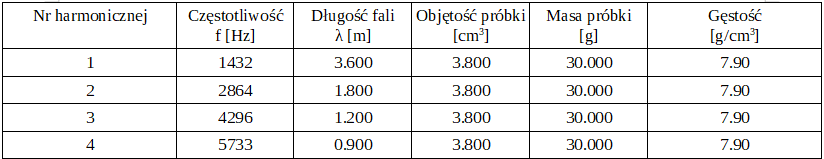
\includegraphics[width=16cm]{stal}
\caption*{\textbf{Tab. 1}: Wyniki pomiarów dla stalowego pręta}
\end{figure} 
\begin{figure}[H]
\centering
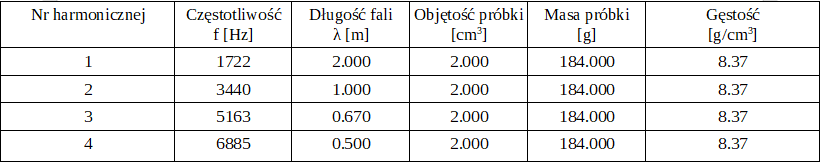
\includegraphics[width=16cm]{mosiadz}
\caption*{\textbf{Tab. 2}: Wyniki pomiarów dla mosiężnego pręta}
\end{figure} 
\begin{figure}[H]
\centering
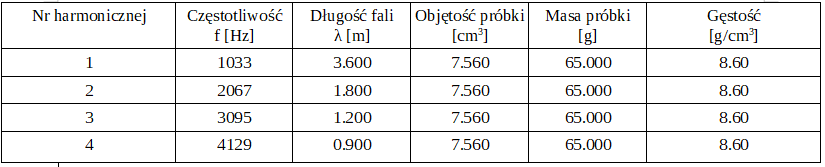
\includegraphics[width=16cm]{miedz}
\caption*{\textbf{Tab. 3}: Wyniki pomiarów dla miedzianego pręta}
\end{figure} 
\begin{figure}[H]
\centering
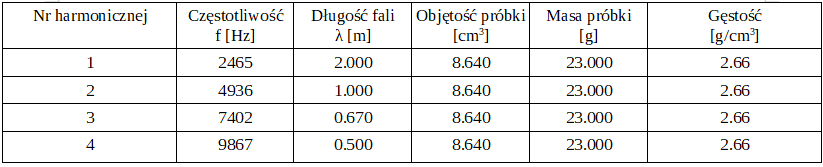
\includegraphics[width=16cm]{aluminium}
\caption*{\textbf{Tab. 4}: Wyniki pomiarów dla aluminiowego pręta}
\end{figure} \newpage
\section{Opracowanie wyników pomiarów}
\subsection{Wyznaczenie gęstości prętów użytych w ćwiczeniu}
Przy pomocy miarki w rolce oraz suwmiarki zmierzyliśmy wymiary geometryczne odpowiednich próbek materiałów. Niepewność miarki przyjęliśmy działkę elementarną $1\;mm$, zaś niepewność suwmiarki przyjęliśmy $0.1\;mm$. Następnie zważyliśmy próbki używając wagi elektronicznej, której niepewność przyjęliśmy równą $0.001\;g$. Gęstość obliczyliśmy używając wzoru $\rho=\frac{m}{V}$. Dla prętu kwadratowego wzór ten przyjmuje postać $\rho=\frac{m}{a^2H}$, gdzie $a$-długość podstawy kwadratu, $H$-długość pręta, zaś dla okrągłego prętu $\rho=\frac{m}{\pi{r^2}H}$, gdzie $r$-długość promienia okręgu. Przykładowo, dla drutu stalowego, zmierzone wartości: $a=0.35\;cm$,$H=31\;cm$,$m=30\;g$. Wartość gęstości stali wyniosła więc:
\begin{center}
\Large $\rho=\frac{m}{a^2H}=\frac{30\;g}{0.35^2\;cm^2*31\;cm}=7.90\frac{g}{cm^3}$
\end{center}
Wartości gęstości mosiądzu, miedzi oraz aluminium wyniosły kolejno $8.37\frac{g}{cm^3}$, $8.60\frac{g}{cm^3}$, $2.66\frac{g}{cm^3}$. Niepewność pomiarową obliczyliśmy przy pomocy prawa przenoszenia niepewności wyrażonej wzorem:
\begin{center}
\Large $u_c(y)=\sqrt{\sum\limits_{k} [\frac{\partial{y}}{\partial{x_k}}u(x_k)]^2}$
\end{center}
W naszym przypadku wzór przyjmuje postać:
\begin{center}
\Large $u_c(\rho)=\sqrt{[\frac{\partial{\rho}}{\partial{m}}u(m)]^2
+[\frac{\partial{\rho}}{\partial{a}}u(a)]^2+[\frac{\partial{\rho}}{\partial{H}}u(H)]^2}=\sqrt{[\frac{u(m)}{a^2H}]^2
+[\frac{-2mu(a)}{a^3H}]^2+[\frac{-mu(H)}{a^2H^2}]^2}$
\end{center}
Dla stali wartość niepewności pomiarowej wyniosła:
\begin{center}
\Large $u_c(\rho)=\sqrt{[\frac{u(m)}{a^2H}]^2+[\frac{-2mu(a)}{a^3H}]^2+[\frac{-mu(H)}{a^2H^2}]^2}
	=\sqrt{(\frac{0.001\;g}{0.35^2\;cm^2*31\;cm})^2+(\frac{-2*30\;g*0.01\;cm}{0.35^3\;cm^3*31\;cm})^2
	+(\frac{-30\;g*0.1\;cm}{0.35^2\;cm^2*31^2\;cm^2})^2}=0.45\frac{g}{cm^3}$
\end{center}
Wartości niepewności pomiarowych dla mosiądzu,miedzi oraz aluminium to kolejno $0.17\frac{g}{cm^3}$, $0.27\frac{g}{cm^3}$, $0.08\frac{g}{cm^3}$.
Niepewności rozszerzone dla $k=2$ wynoszą zaś kolejno $0.9\frac{g}{cm^3}$, $0.34\frac{g}{cm^3}$, $0.54\frac{g}{cm^3}$, $0.16\frac{g}{cm^3}$.
\subsection{Wyznaczenie prędkości fali podłużnej w pręcie}
Jako niepewność pomiaru długości fali przyjęliśmy działkę elementarną miarki $u(\lambda)=1\;mm$, zaś jako niepewność pomiaru częstotliwości przyjęliśmy 
$u(f)=5\;Hz$. Wartość prędkości każdej harmonicznej obliczyliśmy ze wzoru $v=2lf=\lambda{f}$. Dla pierwszej harmoniczej fali wytworzonej \newline w stalowym pręcie:
\begin{center}
\Large $v=\lambda{f}=3.6\;m*1432\;Hz\approx5155.20\;\frac{m}{s}$
\end{center}
Niepewność prędkości wyznaczyliśmy przy pomocy prawa przenoszenia niepewności:
\begin{center}
\Large $u(v)=\sqrt{[\frac{\partial{v}}{\partial{\lambda}}u(\lambda)]^2+[\frac{\partial{v}}{\partial{f}}u(f)]^2}$
\end{center}
Dla pierwszej harmonicznej fali wytworzonej w stalowym pręcie:
\begin{center}
\Large $u(v)=\sqrt{[f*u(\lambda)]^2+[\lambda*u(f)]^2}=\sqrt{(1432\;Hz*0.001\;m)^2+(3.6\;m*5\;Hz)^2}\approx18.06\;\frac{m}{s}$
\end{center}
Pozostałe wyniki, obliczone w identyczny sposób, wpisane zostały do tabel na następnej stronie. \newline
Wartość średnia prędkości nie zależy od częstotliwości ani od wymiarów geometrycznych i kształtu przekroju pręta. Można więc obliczyć ją jako średnią arytmetyczną wszystkich wartości. Przykładowo, wartość prędkości dla fali w stalowym pręcie wyniosła:
\begin{center}
\Large $v_{śr}=\frac{v_1+v_2+v_3+v_4}{4}=\frac{5155.2\;\frac{m}{s}+5155.2\;\frac{m}{s}+5155.2\;\frac{m}{s}+5159.7\;\frac{m}{s}}{4}=5156.33\;\frac{m}{s}$
\end{center}
Wartości średniej prędkości dla mosiądzu, miedzi oraz aluminium to kolejno $3446.43\;\frac{m}{s}$, $3717.38\;\frac{m}{s}$, $4939.71\;\frac{m}{s}$.
\subsection{Wyznaczenie wartości modułu Younga}
Przy pomocy obliczonych wartości gęstości $\rho$, długości fali $\lambda$ oraz częstotliwości $f$ jesteśmy w stanie obliczyć wartość modułu Younga używając wzoru:
\begin{center}
\Large $E=\rho\lambda^2f^2$
\end{center}
Dla pierwszej harmonicznej fali wytworzonej w stalowym pręcie: 
\begin{center}
\Large $E=7900\;\frac{kg}{m^3}*(3.6\;m)^2*(1432\;Hz)^2= 2.094*10^5\;MPa$
\end{center}
Niepewność pomiaru wartości modułu Younga wyznaczliśmy przy pomocy prawa przenoszenia niepewności:
\begin{center}
\Large $u(E)=\sqrt{[\frac{\partial{E}}{\partial{\rho}}u(\rho)]^2+[\frac{\partial{E}}{\partial{\lambda}}u(\lambda)]^2
+[\frac{\partial{E}}{\partial{f}}u(f)]^2}$
\end{center}
W naszym przypadku:
\begin{center}
\Large $u(E)=\sqrt{[\lambda^2f^2u(\rho)]^2+[2\rho\lambda{f}^2u(\lambda)]^2
+[2\rho\lambda^2fu(f)]^2}$
\end{center}
Dla pierwszej harmonicznej fali wytworzonej w stalowym pręcie: 
\begin{center}
\scriptsize $u(E)=\sqrt{[(3.6\;m)^2*(1432\;Hz)^2*450\;\frac{kg}{m^3}]^2+[2*7900\;\frac{kg}{m^3}*3.6\;m*(1432\;Hz)^2*0.001\;m]^2 
+[2*7900\;\frac{kg}{m^3}*(3.6\;m)^2*1432\;Hz*5\;Hz]^2}=0.121*10^5\;MPa$
\end{center}
Pozostałe wyniki, obliczone w identyczny sposób, wpisane zostały do tabel na następnej stronie. \newline
\begin{figure}[H]
\centering
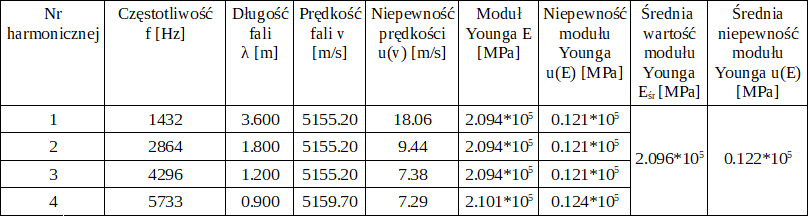
\includegraphics[width=16cm]{wyniki1}
\caption*{\textbf{Tab. 5}: Wyniki pomiarów dla stalowego pręta}
\end{figure} 
\begin{figure}[H]
\centering
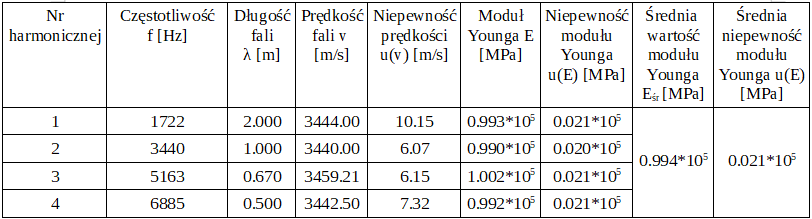
\includegraphics[width=16cm]{wyniki2}
\caption*{\textbf{Tab. 6}: Wyniki pomiarów dla mosiężnego pręta}
\end{figure} 
\begin{figure}[H]
\centering
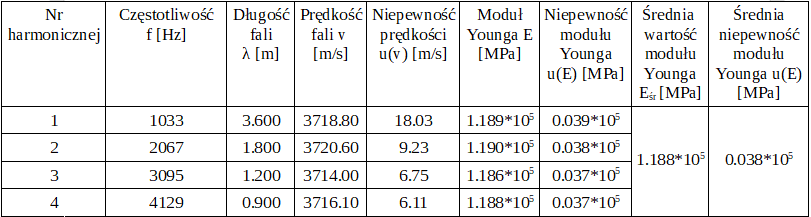
\includegraphics[width=16cm]{wyniki3}
\caption*{\textbf{Tab. 7}: Wyniki pomiarów dla miedzianego pręta}
\end{figure} 
\begin{figure}[H]
\centering
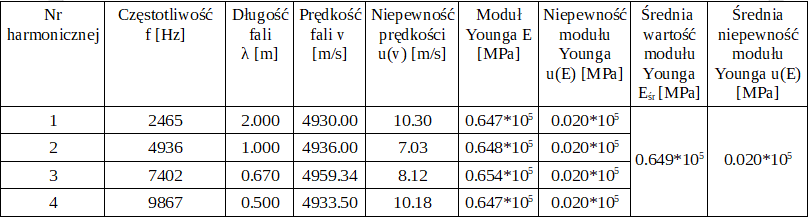
\includegraphics[width=16cm]{wyniki4}
\caption*{\textbf{Tab. 8}: Wyniki pomiarów dla aluminiowego pręta}
\end{figure} \newpage
\noindent Policzyliśmy również średnią wartość modułu Younga $E_{sr}$ oraz średnią wartość niepewności modułu Younga $u(E)$ jako średnią arytmetyczną wszystkich wyników. Przykładowo, dla stali średnia wartość modułu Younga wyniosła:
\begin{center}
\Large $E_{sr}=\frac{E_1+E_2+E_3+E_4}{4}=\frac{(2.094+2.094+2.094+2.101)*10^5\;MPa}{4}=2.096*10^5\;MPa$
\end{center}
Średnia wartość niepewności wyniosła zaś:
\begin{center}
\Large $u(E)=\frac{u(E_1)+u(E_2)+u(E_3)+u(E_4)}{4}=\frac{(0.121+0.121+0.121+0.124)*10^5\;MPa}{4}=0.122*10^5\;MPa$
\end{center}
Pozostałe wyniki, obliczone w identyczny sposób, wpisane zostały do tabel. \newline
Obliczyliśmy również średnie niepewności względne. Przykładowo, dla stali wyniosła ona:
\begin{center}
\Large $\frac{u(E)}{E_{sr}}=\frac{0.122*10^5\;MPa}{2.096*10^5\;MPa}=0.058=5.8\%$
\end{center}
Średnie niepewności względne dla mosiądzu, miedzi oraz aluminium to kolejno $2.1\%$, $3.2\%$, $3.1\%$.
\section{Wnioski}
Wyniki dla stali, mosiądzu oraz miedzi po uwzględnieniu niepewności pomiarowych okazały się zgodne z tabelarycznymi. Wartość modułu Younga dla aluminium nieznacznie odbiega od wartości tabelarycznej. Otrzymane wyniki pozwalają stwierdzić, że wykonane doświadczenie to całkiem dobra metoda znalezienia wartości modułu Younga. Wyniki aluminium nie okazały się tak dokładne jak inne, ponieważ pręt wykonany z tego materiału był bardzo lekki i cienki co utrudniło nam poprawne przystawienie mikrofonu do jednego z końców pręta. Również całkiem niemałe niepewności względne pokazują, że nie jest to idealny sposób pomiaru wartości modułu Younga a bardzo bliskie wyniki mogły być kwestią przypadku. Doświadczenie potwierdziło również, że umieszczenie ściskacza w miejscach, gdzie teorytycznie powinny powstać węzły dla kolejnych harmonicznych, faktycznie te węzły utworzyło.
\begin{figure}[H]
\centering
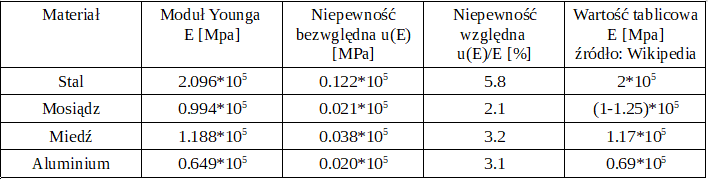
\includegraphics[width=16cm]{podsumowanie}
\caption*{\textbf{Tab. 9}: Podsumowanie wyników}
\end{figure} 
\end{document}
